\subsection*{Diseño VLSI}


En este proceso se detalla el diseño y la fabricación de los CMOS, con el fin de poder fabricar un chip. Este proceso requiere de los transistores de canal n (nMOS) y canal p (pMOS).
Estos sistemas basados en VLSI contienen grandes ventajas en el mundo de la electrónica, ya que permiten hacer chip con muchas funcionalidades a un tamaño muy pequeño, La velocidad también se considera un factor importante, ya que las capacitancias parásitas se logran reducir a un nivel considerable y por último la potencia se logra reducir, en donde se puede ver beneficiado respecto al costo, alimentación más pequeña, enfriamiento, etc.

Desde que William Schockley, John Bardeen y Walter Brattain logra inventar el transistor de puntas de contacto, comenzaron a revolucionar este mundo de los transistores y al proponer el transistor bipolar en 1948, es una de las grandes bases que se utiliza en la actualidad, para realizar el proceso de un chip a nano escala. 
Luego de los años se descubrió la estructura de los MOSFET'S que llegaron a reemplazar a los JFET'S, esto fue gracias a Ian Munro Ross. La idea de los MOSFET'S era más antigua pero el logro que se hiciera viable los efectos de campo.
El VLSI se conoce como \textit{Very Large Scale Integration}, en donde el número de componentes es de 10,000 a 100,000 y el número de compuertas es de 1000 a 10,000. 

El ingeniero Gordon Moore, logro observar en 1965 que la cantidad de transistores iba aumentando según los años que pasaban por un factor de 2, es decir que por cada año la cantidad de transistores en un microprocesador aumentaba cada año. En el 2007, el mismo Moore produjo que su ley dejara de existir dentro de 10 o 15 años, dependiendo de lo que se realice en estos años.

\cite{hoover2010bio} \cite{park2014design}


\subsection*{Flujo de diseño}


El flujo de diseño nos muestra los pasos requeridos para poder realizar una serie de pasos para el diseño y la fabricación de lo que es un circuito integrado. Este flujo de diseño se logra dividir en 2 partes (Front End y Back End). Lo que se busca con este flujo es encontrar la manera que, a la hora de fabricar un chip no tenga errores y que sea funcional respecto a las necesidades requeridas.


 \textbf{Front End}
 Este se encarga de resolver un problema pasándolo a un lenguaje descriptivo, en este caso se usa los lenguajes de Verilog y VHDL. 
 En esta etapa se encuentran los pasos necesarios para la arquitectura de diseño. A continuación, se logran ver los pasos necesarios para que se pueda elaborar el diseño front end.
 
 \underline{Primero}: Se debe realizar el circuito, por medio del lenguaje descriptivo de hardware como Verilog, el cual presenta la solución del problema establecido.
 
 \underline{Segundo}:  Se denomina la síntesis lógica, este es un proceso en donde se toma el diseño RTL, que fue descrito en Verilog o VHDL. En esta también se producen comprobaciones y simulaciones, con el fin de comprobar el modelo RTL propuesto.
 
 \underline{Tercero}: El netlist, este es un circuito generado, después de la síntesis lógica en donde se logra observar  por medio de librerías.
 
 \underline{Cuarto}: El Ultimo paso, se utilizan varios softwares con el fin de verificar la funcionalidad de la síntesis del circuito.


 \cite{charls} 


 \begin{figure}[h]
    \centering
    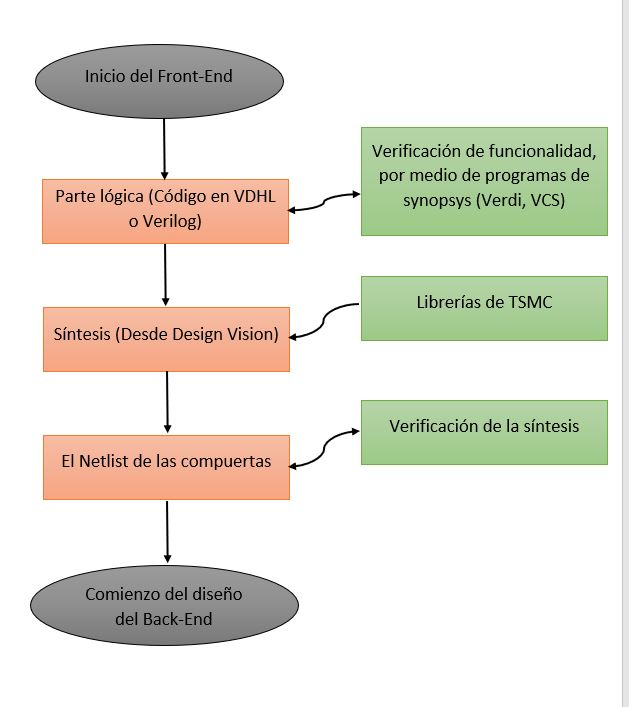
\includegraphics[width=0.58\textwidth]{figuras/Font.JPG}
    \caption{Diagrama del Front-End}
    \label{fig:mesh1}
\end{figure}
 
 

 
 
 \textbf{Back End} 
Esta parte va más inclinada a la implementación del circuito en físico. Esta toma la parte del lenguaje descriptivo, en forma de un diseño en físico, el cual se convierte en un layout, en donde podemos ver a más detalle como está compuesto el circuito.

\underline{Primero}: En este se encuentra la síntesis física, el cual se basa en el netlist. Al pasar a esta etapa se encuentra el layout, en donde tenemos más información acerca del circuito y además podemos manipularlo, con el fin que cumpla las reglas de diseño especificadas por la empresa que va a realizar el chip.

\underline{Segundo}: Obtenemos lo que es el Placement, en este caso nosotros decidimos donde se van a poner las celdas con el fin de que llegue a ser lo más óptimo posible y sencillo de arreglar en un futuro.

\underline{Tercero}: Al tener las celdas puestas en la mejor posición posible se procede a interconectar las salidas y las entradas de cada parte del circuito descrito, este parte se conoce como routing.

\underline{Cuarto}: Este se denomina \textit{Design Rule Check}, este consiste en verificar que el layout no contenga errores o reglas de diseño que son impuestas dependiendo de la tecnología.

\underline{Quinto}: Este se denomina \textit{layout versus schematic}, este consiste en verificar la integridad del diseño. Este compara el layout con el netlist (Síntesis lógica).

\underline{Sexto}: La extracción de parásitos, aquí es donde se simula la parte del layout con la cantidad de parásitos que pueda tener el layout, y se logra ver que tanto llega a afectar al final del proceso.


 \cite{charls} 
\begin{figure}[h]
    \centering
    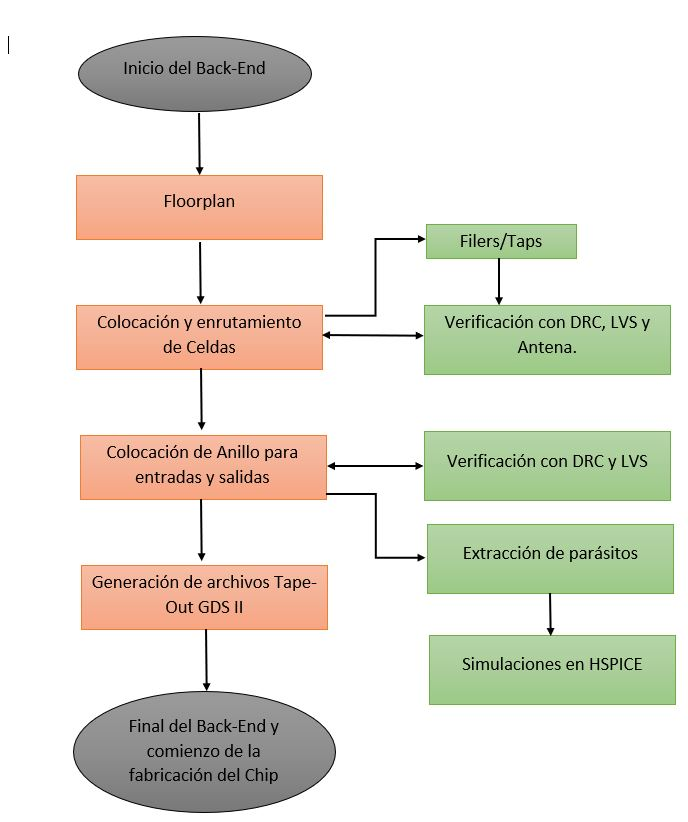
\includegraphics[width=0.57\textwidth]{figuras/Back.JPG}
    \caption{Diagrama del Back-End}
    \label{fig:mesh1}
\end{figure}
\newpage

\subsection*{Lenguaje Descriptor de Hardware}

Estos lenguajes son los que son utilizados con el fin de describir una arquitectura y lograr visualizar el comportamiento de un sistema electrónico. 
La forma más fácil de representar un circuito es mediante la utilización de diagramas o esquemas estos hacen una representación gráfica de lo que se pretende realizar. 
Con el tiempo comenzaron a salir circuitos más complejos que ya no podían ser representadas de una manera visual, por lo que nació una idea de integrar las herramientas de descripción de síntesis, simulación y realización. Al principio se logró utilizar un lenguaje de descripción que solo permitía secuencias simples, a este se le nombro Netlist. Luego de estos programas simples que ya eran reconocidos como lenguajes de descripción de hardware, se logró ver el gran impacto que podían tener a la hora de describir circuitos complejos.

Mientras que todo iba evolucionando, la posibilidad de desarrollar circuitos digitales mediante dispositivos programables era la forma más viable, ya que los circuitos, ya representaban una cantidad considerable de componentes. Este tipo de lenguajes estaban orientados para la realización de simulaciones, por lo que no importaba mucho que el nivel de abstracción fuera tan alto. Al momento de la aparición de técnicas para la síntesis de circuitos a partir de lenguajes que se consideraban de alto nivel de abstracción, se comenzaron a utilizar para la síntesis de circuitos.

\cite{DDH} 

\subsection*{Verilog y VHDL}

Verilog es un lenguaje que se utiliza para describir hardware, en el cual podemos diseñar y simular circuitos electrónicos (Digitales). Este lenguaje es una derivación de la programación en C, con el fin que los ingenieros puedan entenderlo. 
 VHDL también se encuentra englobado dentro de los lenguajes de descripción de Hardware. En si, un HDL es un tipo de lenguaje especializado que define la estructura, diseño, operación de circuitos electrónicos y circuitos digitales.
 Este tipo de lenguaje es una forma de representación formal de un circuito electrónico, con la posibilidad de hacer un proceso más simple.
 
 EL lenguaje VHDL se considera un estándar, este no depende de ningún fabricante o dispositivo, es independiente. El fin de este lenguaje es que se puedan reutilizar los diseños y tiene la ventaja de ser un diseño jerárquico.  Verilog este puede llegar a soportar lo que son circuitos analógicos, pruebas y señales mixtas a distintos niveles de abstracción.

 \cite{DDH} 

\subsection*{VCS}

Es una de las soluciones de la verificación funcional que se utiliza en la mayoría de las empresas de semiconductores en el mundo. Este es un programa que proporciona características innovadoras para lograr un mayor rendimiento y permite los flujos de verificación de desplazamiento al principio del ciclo de diseño.
Este ofrece como solución con Native Testbench, compatibilidad con Verilog, análisis y cobertura e integración con Verdi. VCS satisface las necesidades de los diseñadores para poder verificar los resultados obtenidos de la prueba de un circuito elaborado en un programa compatible de descripción de hardware.

Esta herramienta cuenta con un flujo de dos pasos para evaluar el funcionamiento del circuito descrito.

 \cite{VCS} 

 
  \textbf{Flujos de VCS}  
  
  
  Este es un flujo que se utiliza para poder comprobar si el diseño en Verilog HDL y SystemVerilog, son funcionales para la fabricación del Chip.
  
  \underline{Primero}:  El primer paso es lograr compilar el diseño, en esta etapa VCS logra construir una instancia de jerarquía y logra generar un archivo .simv que se utiliza para poder realizar la simulación.
  
  \underline{Segundo}:En esta etapa se simula el diseño con el archivo generado en la primera parte (.simv). En esta etapa se logra ver si se logró correr la simulación.
  
  Existe otro flujo de dos pasos, este permite diseños en Verilog, VHDL y mixedHDL. Este consta de 3 pasos.
  
  \underline{Primero}:  Analizar el diseño, en esta etapa VCS logra dar los ejecutables, los cuales son vhdlan y clogan, con el fin de analizar el diseño y lograr almacenar archivos en la carpeta de trabajo.
  
  \underline{Segundo}: Elaborar el diseño, en esta parte se adquiere un archivo .vcs, el cual se compila y logra elaborar el diseño utilizando los archivos generados en la librería de trabajo. Luego da un archivo .simv.
  
  \underline{Tercero}: Simular el diseño, este se logra simular con el archivo, el cual es un ejecutable binario que se describió en el paso anterior.

 \cite{Jeff} 
  
  \subsection*{Verdi}
 Esta herramienta de Synopsys se considera un sistema de depuración automatizado y esta herramienta permite la depuración integral de todos los flujos de diseño y verificación.  Este sistema tiene una tecnología poderosa que le ayuda a comprender el comportamiento del diseño definido, y lo más relevante es que ayuda a optimizar los procesos difíciles y tediosos.
  
  En esta herramienta se reducir el tiempo de depuración en más del 50 por ciento, esto es posible porque automatiza el comportamiento, por medio de un seguimiento con una tecnología única de análisis. También logra extraer, aislar y mostrar la lógica pertinente en los diseños. Logra revelar el funcionamiento y la interacción con el diseño propuesto.
  El sistema de depuración por completo que tiene Verdi, utiliza la tecnología y las capacidades de un sistema de depuración, cabe resaltar que este utiliza funciones avanzadas de depuración con soporte para una gran cantidad de lenguajes y metodologías.

  \cite{verdi} 
  \textbf{Funciones principales}  
  
  \begin{itemize}
   \item Seguimiento rápido de la actividad de muchos ciclos de reloj con una potente tecnología de análisis.
    \item Vistas de flujo temporal que proporciona una visualización de tiempo y estructura para comprender las relaciones de causa y efecto.
    \item Analizar diseños en niveles más altos de abstracción.
    \item Depuración basada en aserciones con soporte integrado.

\end{itemize}

\textbf{Depuración de SystemVerilog Testbench}

\begin{itemize}
    \item Soporte de código fuente para SystemVerilog Testbench, incluyendo la metodología de verificación universal (UVM).
    \item Vistas especializadas que ayudan a comprender el código, viendo la navegación y exploración de jerarquías basadas en declaraciones.
    \item Capacidad de registro de transacciones automatizadas, que brindan una imagen completa de la actividad del banco de pruebas en el entorno de verificación después de la simulación.
    \item Control de simulación interactivo que permite correr el código completo.
    \item Las vistas de depuración compatibles con UVM permite explorar los resultados de aspectos específicos.
    \item Vistas de depuración a nivel de transacción y logran admitir el registro de datos.
\end{itemize}

 \cite{Jeff} 

\textbf{Mas acerca de Verdi}


Este sistema de depuración automatizado tiene compiladores e interfaces.
Los compiladores que son utilizados en la parte de diseño mayoritariamente son Verilog, VHDL Y System Verilog. La interfaz que tiene Verdi implementa los estándares industriales de datos VCD y SDF. Normalmente los resultados por la herramienta son guardados en la Fast Signal Database.  Verdi también permite la interoperabilidad con lo que se conocen los simuladores lógicos, las herramientas de verificación y los análisis de tiempo.

Las bases de datos que Verdi maneja son las de conocimiento que se pueden llamar KDB y la base de datos de señal rápida conocida como FSDB. En KDB normalmente se utiliza para almacenar información lógica y funcional para el diseño implementado.
La base de datos FSDB, logra almacenar los resultados de la simulación.

Al utilizar la información que proporcionan estas bases de datos, Verdi tiene unas herramientas de análisis que resultan ser muy útiles dependiendo de la aplicación que se quiera dar, estas son: Análisis de estructura, comportamiento, evaluación y Mensajes.



 \subsection*{Extracción de parásitos}
La extracción de parásitos se puede realizar después de haber hecho las pruebas pertinentes en el flujo del diseño, este pertenece a la parte del Back-End y se puede realizar correctamente después de realizar el lvs y el drc, que son parte del diseño del layout después con HSPICE se busca el archivo generado con parásitos para ver cómo se comporta la simulación, en donde también se utiliza el StarRc. Todo esto es con el fin de garantizar que el diseño VLSI es factible y que las capacitancias parásitas no van a afectar el circuito.

Esto sucede al jugar con los transistores que generan lo que se llaman capacitancias parásitas que generan un efecto adicional en los conductores que funcionan como placas entre el dieléctrico, y este tipo de parásitos va a ir aumentando conforme las frecuencias, más que todo en este caso al meter muchos transistores las capacitancias parásitas van a ir aumentando.  En la implementación de circuitos nanométricas las interconexiones entre cables pueden llegar a representar problemas por los parásitos que se pueden generar, al igual que puede pasar con las difusiones de los componentes que pueda proveer las librerías de TSMC.

El fin de la extracción de parásitos es la representación de los efectos electromagnéticos que los cables y las difusiones puedan generar al momento de correr la simulación, en componentes como la capacitancia, resistencia e inductancia.

 \cite{charls} 

  \subsection*{StarRC}

Esta herramienta se considera la solución para la extracción de parásitos. Esta herramienta amplia los beneficios de rendimiento, en donde se basa en mejorar la arquitectura y hace que el proceso sea más efectivo. Este programa logra eliminar la necesidad de lo que es la escritura parásita en un netlist y este mismo logra ahorrar el espacio del disco. Mas que todo se especializa en optimizar el proceso reduciendo las capacitancias parásitas que puedan llegar a afectar el comportamiento deseado de un circuito.

 \cite{StarRc} 


\subsection*{HSPICE}
Hspice es una herramienta de synopsys que permite realizar las simulaciones de un programa generado (.spf), en donde viene de la mano con Custom Wave View. El fin de este programa es ver una simulación y lograr ver el comportamiento del circuito. 
Este se considera uno de los simuladores más potentes, ya que muestra gran precisión en los datos y la mayoría de las empresas de semiconductores dependen de esta herramienta.
Además, se pueden realizar análisis de los circuitos eléctricos en estado estacionario, en el dominio de frecuencia y el transitorio.



 \cite{charls} 



\subsection*{Trabajo realizado}

En los años anteriores se realizaron trabajos de investigación para poder utilizar y lograr entender los softwares como Verdi, Formality, VCS y HSPICE.

Se realizaron diferentes tipos de flujos según la complejidad requerida, en donde se lograron diseñar distintos flujos en la herramienta VCS, con el objetivo de verificar el comportamiento del circuito sintetizado. En este se realizan 2 simulaciones una para el circuito original y uno para el circuito sintetizado que ya hace referencia a las librerías de TSMC de 180 nm. Entonces el trabajo realizado por Jefferson Ruano, ya nos dice las librerías utilizadas para la simulación. En el trabajo del año 2020, también se logra ver el flujo de simulación con detección de condiciones de carrera, las cuales puede mostrar inconsistencias en las simulaciones ejecutadas. También logra mostrar el flujo para la evaluación de desempeño, en donde VCS cuenta con una herramienta conocida como generación de perfiles de simulación unificado, esta herramienta nos permite ver la cantidad de tiempo de CPU y memoria usada por nuestro diseño. 
El trabajo realizado con Formality, se logró aprender que es una alternativa a la validación en las herramientas de VCS y Verdi. Este llega a generar un reporte más practico, ya que logra generar un reporte más simple con las coincidencias e inconsistencias al ver los circuitos.

En el trabajo realizado por Charlie Ayenci, en donde logro simular el diseño con parásitos por medio HSPICE, hubo ciertos errores al correr la simulación en donde, la empresa TSMC solamente logra proveer un kit académico, por lo que solo se encontraran las black boxes, que solo contienen el diseño de silicio del componente y con esto el netlist no logra poseer los puertos de entrada, salida y alimentación.  

 \cite{charls} 
  \cite{Jeff} 